\chapter{Results}
\label{chapter:results}

\section{Cache-oblivious B-tree}
We found the performance of cache-oblivious B-trees very competitive compared
to B-trees on both random uniform access patterns and modestly large working
sets. As seen on figure \ref{fig:cob-performance}, random \textsc{Find}s
were up to twice as fast in large cache-oblivious B-trees without ever being
significantly slower on small dictionaries.
The large density of the van Emde Boas tree is the likely reason for these
gains.

\textsc{Insert} operations, however, are comparatively slow in
smaller cache-oblivious B-trees (e.g.\ $\leq$ 100~000 keys). We believe
this slowdown is probably due to the cost of rebuilds, which properly
amortizes away only on larger dictionaries. A smarter choice of tuning
constants (i.e.\ the minimum and maximum density and piece sizes) might
make updates of smaller dictionaries more efficient.

\begin{figure}
\centering
\begin{subfigure}[b]{0.45\textwidth}
	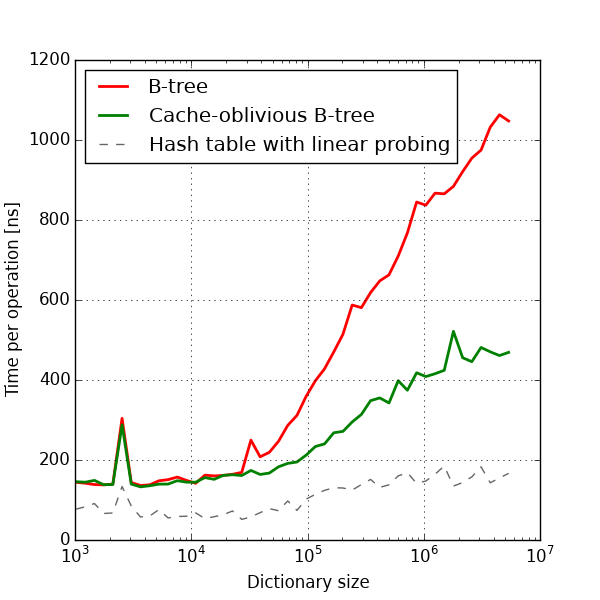
\includegraphics[width=\textwidth]{img/performance/cob-performance-1}
	\caption{Random \textsc{Find}s}
\end{subfigure}
~
\begin{subfigure}[b]{0.45\textwidth}
	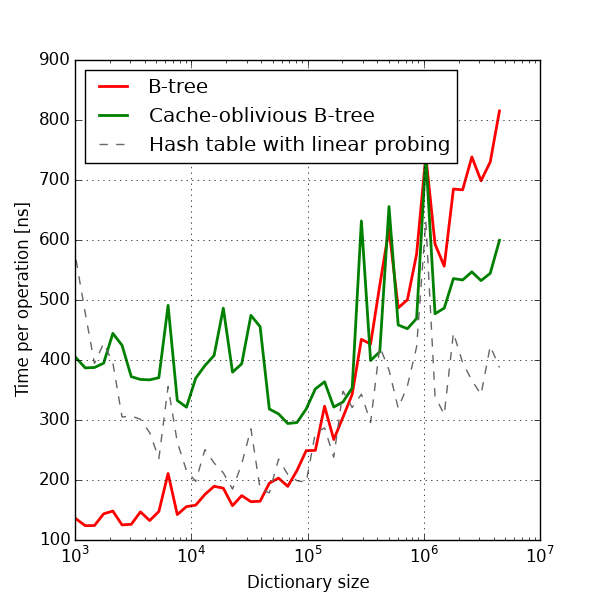
\includegraphics[width=\textwidth]{img/performance/cob-performance-2}
	\caption{Random \textsc{Insert}s}
\end{subfigure}
~
\begin{subfigure}[b]{0.45\textwidth}
	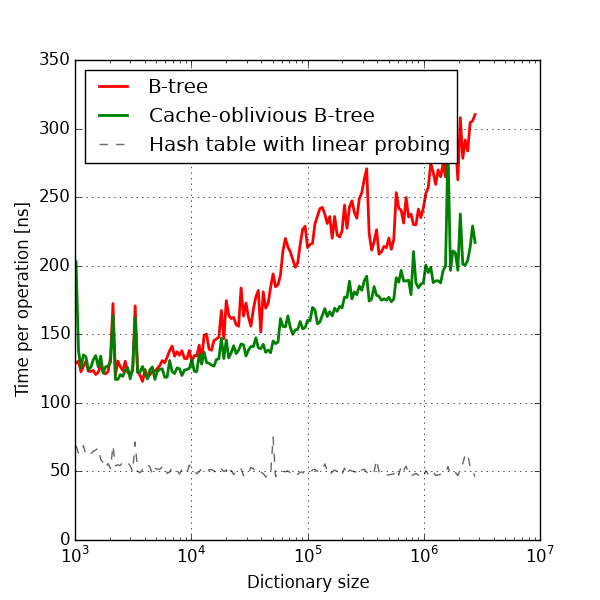
\includegraphics[width=\textwidth]{img/performance/cob-performance-3}
	\caption{\textsc{Find}s, working set of 1~000 keys}
\end{subfigure}
~
\begin{subfigure}[b]{0.45\textwidth}
	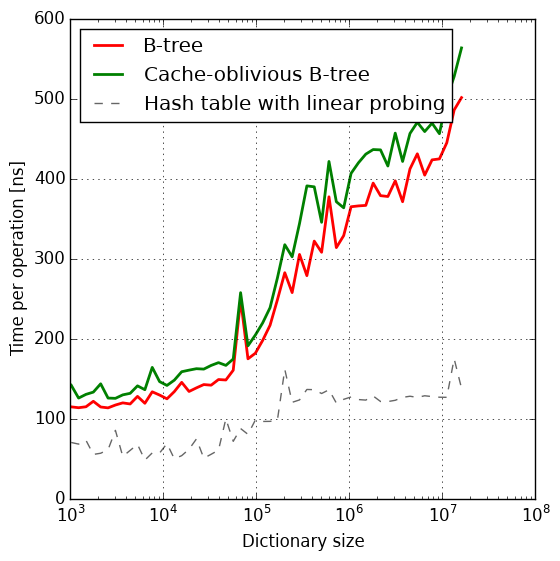
\includegraphics[width=\textwidth]{img/performance/cob-performance-4}
	\caption{\textsc{Find}s, working set of 100~000 keys}
\end{subfigure}

\begin{subfigure}[b]{0.45\textwidth}
	TODO
	\caption{Word occurrence counting}
\end{subfigure}
\caption{Benchmarks of cache-oblivious B-trees.
	Measurements of hash table with linear probing included for reference.}
\label{fig:cob-performance}
\end{figure}

TODO: left-to-right scans: mel bych to implementovat v B-stromech...

These results confirm that cache-oblivious B-trees are a better alternative
to traditional B-trees in larger in-memory databases with frequent
\textsc{Find}s.

\section{Self-adjusting structures}
Splay trees are the canonical self-adjusting structure we would like to
outperfrom. As expected, splay trees are somewhat slower than B-trees on
unpredictable operations (see figure \ref{fig:self-adj-performance}).

\begin{figure}
\begin{subfigure}[b]{0.45\textwidth}
	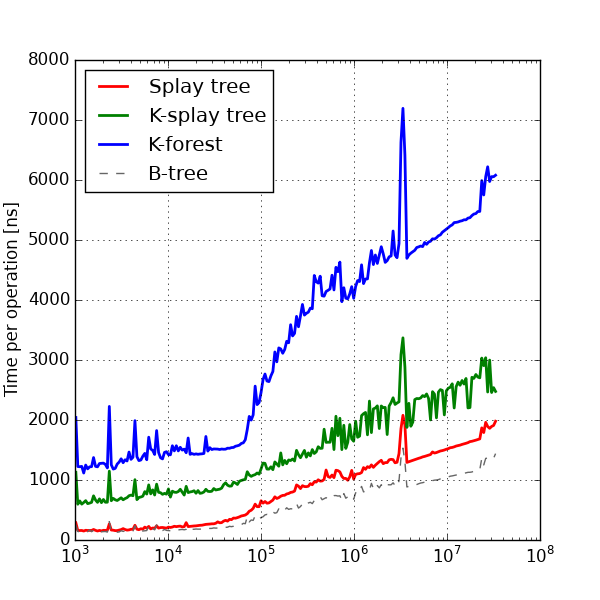
\includegraphics[width=\textwidth]{img/performance/self-adj-random-find}
	\caption{Random \textsc{Find}s}
\end{subfigure}
~
\begin{subfigure}[b]{0.45\textwidth}
	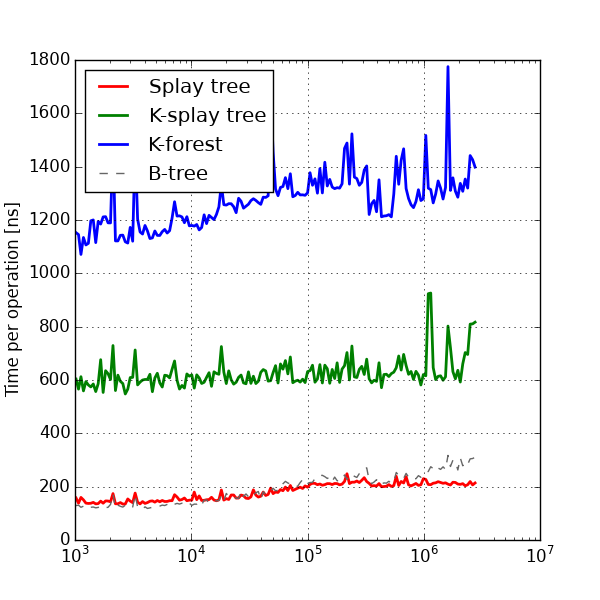
\includegraphics[width=\textwidth]{img/performance/self-adj-ws-1k}
	\caption{\textsc{Find}s, working set of 1~000 keys}
\end{subfigure}
~
\begin{subfigure}[b]{0.45\textwidth}
	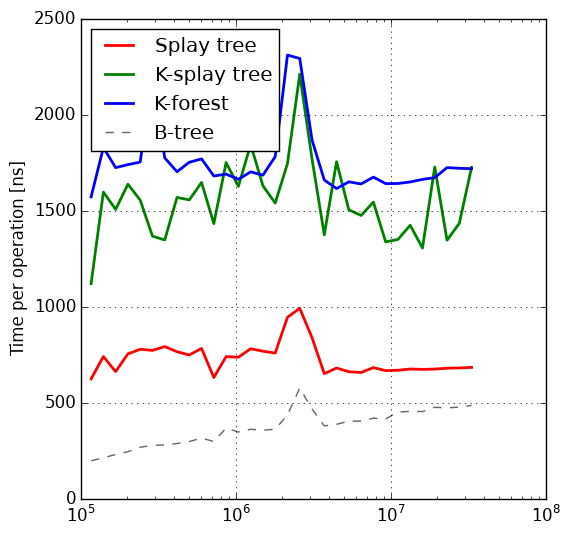
\includegraphics[width=\textwidth]{img/performance/self-adj-ws-100k}
	\caption{\textsc{Find}s, working set of 100~000 keys}
\end{subfigure}
% TODO: inserts, working sets

\caption{Benchmarks of self-adjusting structures.
	B-trees are included for reference.}
\label{fig:self-adj-performance}
\end{figure}

Unfortunately, we found both $k$-splay trees and $k$-forest severely lacking in
performance in every experiment.

FIXME: splay trees are fast
TODO: profile k-splay, find bottleneck

$k$-forests were slow both backed by B-trees and by cache-oblivious B-trees.
Choosing a larger $k$ slightly helped, but larger values of $k$ also degenerate
$k$-forests into their backing structure. As expected, $k$-forests do exhibit
the working set property, but simple structures without the working set property
outperformed $k$-forests several times on working set tests.

\section{Hashing}
FIXME: cuckoo, linear probing is good

\section{Practical experiments}
TODO: cloud experiment results
TODO: Firefox results
